\section{问题二：全过程变物性耦合场模型}

\subsection{变物性带来的结构改变}

全过程计算改用附录 3 给出的一组经验公式，即式~\eqref{eq:app3}。方程形式与问题一完全相同，改变的只是四个系数不再是常数：密度随干基含水率线性变化，比热容与导热系数随湿基含水率变化，扩散系数同时含有含水率因子与温度的 Arrhenius 因子。把实算中真实出现过的三个状态代入可以看出变化幅度。含水率为 $2.55$、$1.00$、$0.15$~kg/kg 时，密度依次为 $976.4$、$778.0$、$669.2$~kg/m$^3$，比热容依次为 $3415.3$、$2818.0$、$1806.9$~J/(kg$\cdot$K)，导热系数依次为 $0.483$、$0.400$、$0.2596$~W/(m$\cdot$K)，扩散系数依次为 $5.642\times10^{-9}$、$7.004\times10^{-9}$、$8.001\times10^{-10}$~m$^2$/s。前三项各自变化不足一倍，仍属同一量级；扩散系数则先随温度上升而增大、再随含水率下降而急剧减小，非单调且跨越一个数量级以上。

系数依赖待求解，方程由线性变为非线性，因此每个时间层内都要用当前解重算物性并迭代到自洽，收敛准则取式~\eqref{eq:picard}。这使求解结构由问题一的单层推进变成双层嵌套，如图~\ref{fig:flow-q2}。

\begin{figure}[htbp]
  \centering
  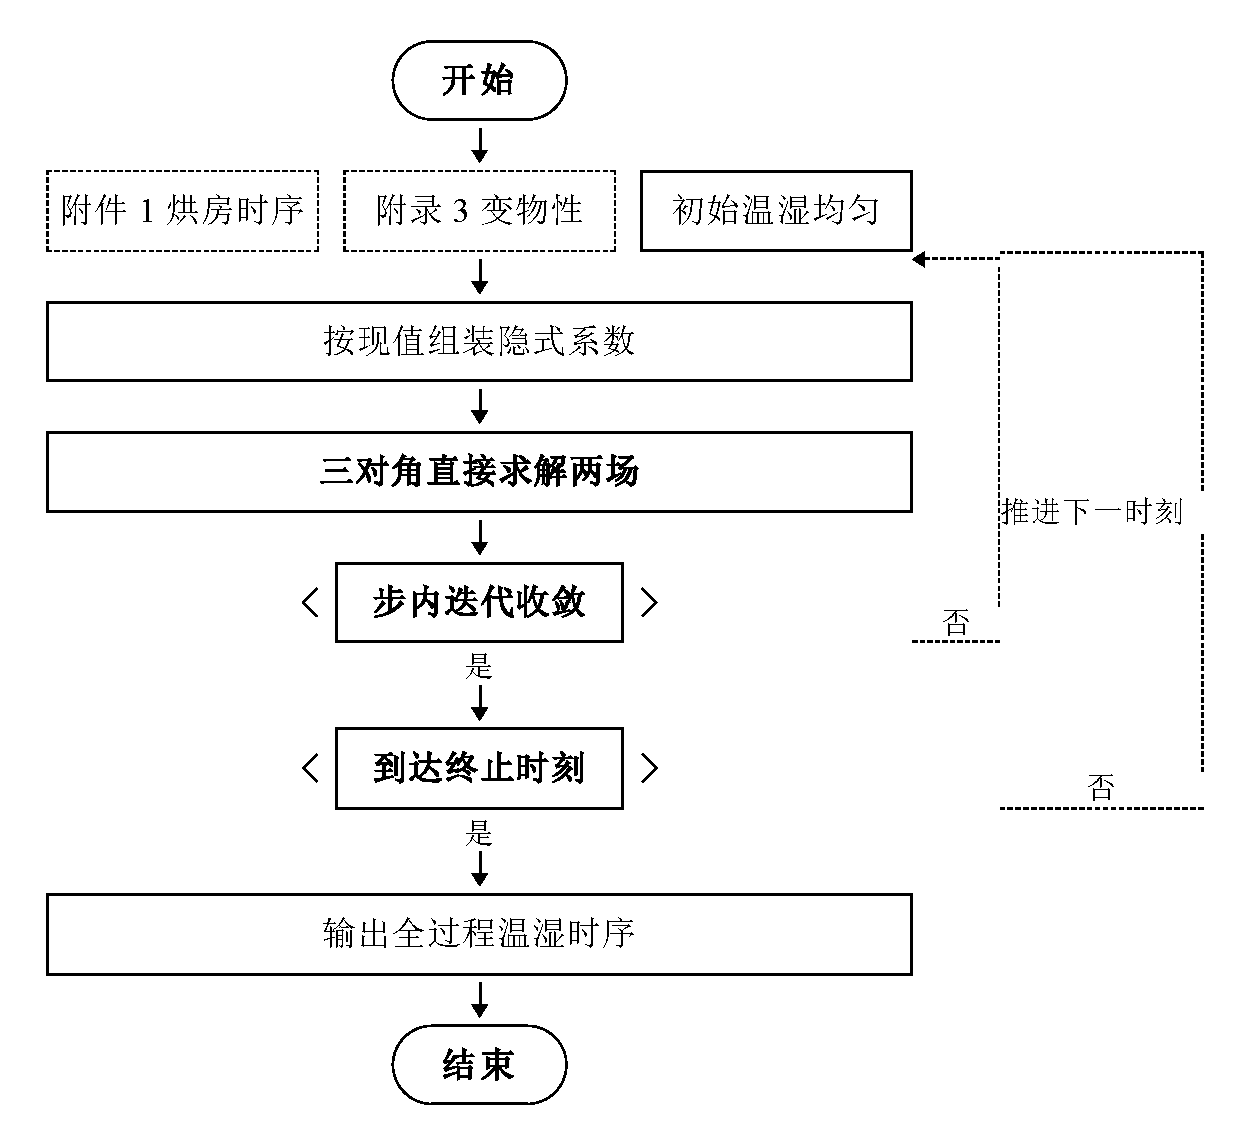
\includegraphics[width=0.86\textwidth,height=0.8\textheight,keepaspectratio]{../figures/fig_flow_q2.pdf}
  \caption{问题 2 全过程求解的双重迭代结构。主链是一次时间步内的动作；内侧回路
  为步内 Picard 非线性迭代，外侧回路为步间时间推进，两条回路都返回到系数组装，
  区别在于外侧回路先推进到下一时刻。虚线框表示题给数据。}
  \label{fig:flow-q2}
\end{figure}

两条回路的区别值得说清：内侧回路不推进时间，它反复在同一时刻上更新系数直至解不再变化，解决的是非线性；外侧回路推进时间，解决的是演化。两者都回到系数组装这一步，因为一旦解或时刻改变，物性和界面系数都必须重算。实算中恒温平台段每步只需三到五次内迭代即收敛，预热段因温度变化快，峰值为 12 次。

\subsection{扩散系数的双变量依赖}

扩散系数第一次同时依赖两个场，它是两个方程之间耦合的唯一通道，其形态决定了整个干燥过程的节奏，因此值得单独考察，见图~\ref{fig:diff-surface}。

\begin{figure}[htbp]
  \centering
  % 本图宽度取 0.93 而非横图默认的 0.90：该图 b 面板的刻度字号在原生画布上只有 8.0pt，
  % 按 0.90 插入后上页字号为 7.75pt，低于 8pt 可读下限；0.93 使其回到 8.01pt。
  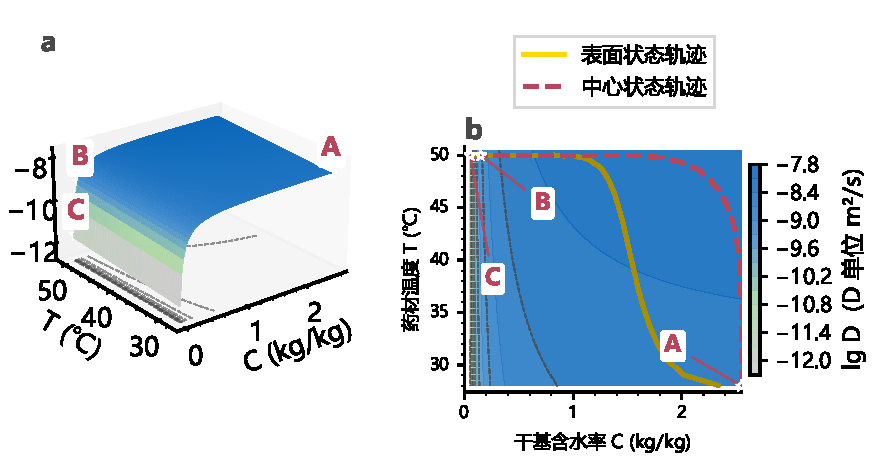
\includegraphics[width=0.93\textwidth,height=0.8\textheight,keepaspectratio]{../figures/fig_diff_surface.pdf}
  \caption{附录 3 扩散系数 $D(C,T)$ 的三维曲面与俯视投影。a：$\lg D$ 在
  $(C,T)$ 平面上的曲面，温度经 Arrhenius 因子起主导作用，含水率的修正相对
  次要；A、B、C 三点为全过程算例实际经过的状态，依次为初始态、含水率降至判据
  阈值时的状态与终态。b：同一函数的等高线俯视图，叠加中心与表面状态点的实算
  轨迹，可见两条轨迹沿温度方向先分离后合拢。}
  \label{fig:diff-surface}
\end{figure}

曲面沿温度方向的抬升幅度明显大于沿含水率方向，这说明升温对加快水分迁移的贡献超过变干对它的抑制，两者在干燥初期同时发生且方向相反。俯视图上中心与表面的两条轨迹在初期迅速分开，因为表面先升温也先变干；进入恒温段后两条轨迹又逐渐靠拢，因为温度趋于一致，差别只剩含水率。这一先分离后合拢的形态解释了为什么干燥速率在初期最快而后期显著放缓：初期是高温与高含水率叠加的有利区间，后期温度已无提升空间而含水率持续下降，扩散系数只能单向减小。

界面系数按式~\eqref{eq:iface} 的积分平均计算。以实算中一对相邻节点为例，两端含水率为 $2.55$ 与 $1.00$，端点扩散系数为 $1.3470\times10^{-8}$ 与 $1.0247\times10^{-8}$~m$^2$/s，积分平均给出 $1.2279\times10^{-8}$~m$^2$/s，严格落在两端点之间，与通量的物理含义一致。

\subsection{前三小时的温度与含水率}

按题目要求给出前三小时每半小时的结果，温度见表~\ref{tab:q2T}。完整分布按每秒、每 $0.1$~cm 输出，覆盖 $1$ 至 $10800$~s 共三小时，与本问所问的时间窗一致；全过程直到烘干结束的逐点分布由后一问以 $60$~s 间隔给出。

\begin{table}[H]
\centering
\caption{3 小时内药材的温度（单位：°C）}\label{tab:q2T}
\begin{tabular}{cccccc}
\toprule
\multirow{2}{*}{时间/h} & \multicolumn{5}{c}{到药材中心的距离/cm}\\
\cmidrule(lr){2-6}
 & 0 & 0.5 & 1 & 1.5 & 2 \\
\midrule
0.5 & 32.1893 & 32.3822 & 32.9660 & 33.9608 & 35.4132 \\
1.0 & 40.3812 & 40.5531 & 41.0601 & 41.8781 & 42.9977 \\
1.5 & 45.8460 & 45.9341 & 46.1923 & 46.6045 & 47.1397 \\
2.0 & 48.4497 & 48.4875 & 48.5980 & 48.7732 & 49.0031 \\
2.5 & 49.4667 & 49.4789 & 49.5134 & 49.5653 & 49.6609 \\
3.0 & 49.8494 & 49.8553 & 49.8745 & 49.9101 & 49.9664 \\
\bottomrule
\end{tabular}
\end{table}

表中五列在三小时末已收敛到同一个数值附近，径向温差不足 $0.12$~°C，温度场至此基本进入准稳态。同一批时刻与位置上的含水率结果列于表~\ref{tab:q2C}。

\begin{table}[H]
\centering
\caption{3 小时内药材的水分浓度（单位：kg/kg）}\label{tab:q2C}
\begin{tabular}{cccccc}
\toprule
\multirow{2}{*}{时间/h} & \multicolumn{5}{c}{到药材中心的距离/cm}\\
\cmidrule(lr){2-6}
 & 0 & 0.5 & 1 & 1.5 & 2 \\
\midrule
0.5 & 2.5499 & 2.5488 & 2.5254 & 2.3259 & 1.6486 \\
1.0 & 2.5255 & 2.4946 & 2.3578 & 2.0231 & 1.4710 \\
1.5 & 2.3859 & 2.3255 & 2.1344 & 1.8020 & 1.3475 \\
2.0 & 2.1708 & 2.1084 & 1.9236 & 1.6259 & 1.2310 \\
2.5 & 1.9566 & 1.9006 & 1.7360 & 1.4719 & 1.1166 \\
3.0 & 1.7662 & 1.7165 & 1.5702 & 1.3332 & 1.0081 \\
\bottomrule
\end{tabular}
\end{table}

两张表的对比清楚显示了两个场的分离。温度在两小时内就基本追上空气温度，第三小时末中心为 $49.8494$~°C、表面为 $49.9664$~°C，中心与表面之差已缩到 $0.12$~°C，整个截面进入准稳态；此后温度不再是限制因素。含水率则完全没有停下来的迹象，三小时末中心仍有 $1.7662$~kg/kg、表面为 $1.0081$~kg/kg，截面平均从 $2.5500$ 降到 $1.3824$~kg/kg，仅完成了到合格阈值所需降幅的一半左右。这一时间尺度的分离是全过程建模的核心事实：温度场很快退居背景，剩下的时间几乎全部花在水分向外扩散上。图~\ref{fig:q2-dual} 把两个场与物性的实时响应画在同一时间轴上。

\begin{figure}[htbp]
  \centering
  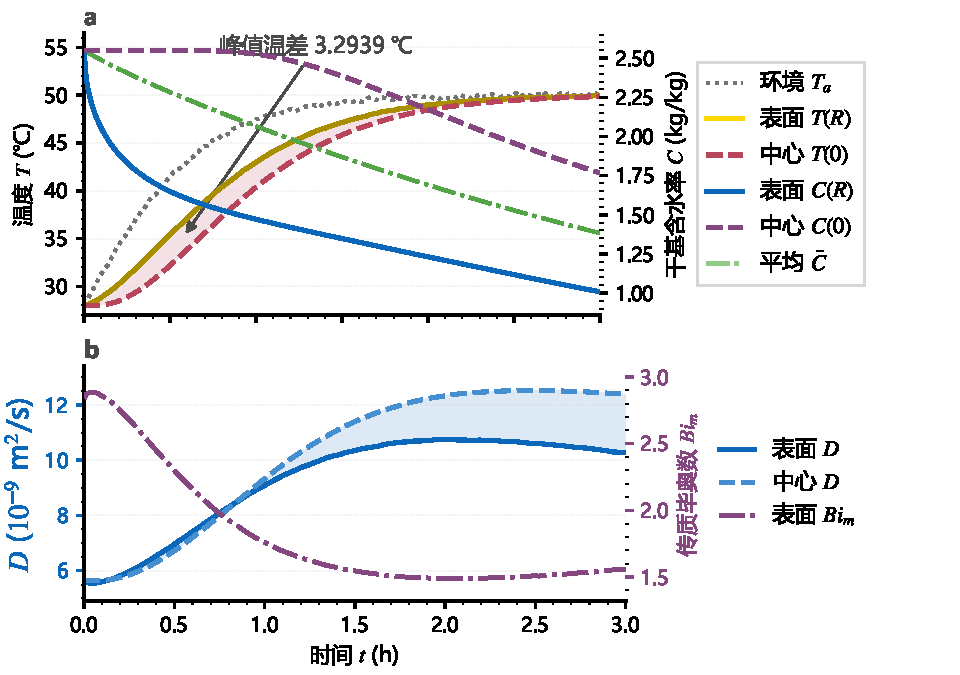
\includegraphics[width=0.9\textwidth,height=0.8\textheight,keepaspectratio]{../figures/fig_q2_dual.pdf}
  \caption{问题 2 前三小时的双轴演化与变物性响应。a：中心与表面温度追随空气
  温度上升，阴影为中心—表面温差带，同期三条含水率曲线同步下降；温度很快进入
  准稳态，含水率的下降贯穿整个过程，两者时间尺度相差一个量级以上。b：表面与
  中心扩散系数、表面传质毕奥数随含水率下降的实时变化，$D$ 在三小时内变化近
  一倍，故变物性不能用常数近似替代。}
  \label{fig:q2-dual}
\end{figure}

左图中温差阴影带在第一小时最宽而后迅速收窄，与表~\ref{tab:q2T} 中中心与表面之差从 $3.2$~°C 缩到 $0.12$~°C 相符；三条含水率曲线则保持大致平行地下行，未见收敛趋势。右图给出变物性不可用常数替代的直接证据：表面与中心的扩散系数在三小时内变化接近一倍，且两者之间始终存在可观差距；表面传质毕奥数同期持续增大，表明限制环节正在由表面对流向内部扩散转移。若把扩散系数冻结在任一时刻的取值，整个过程的速率都会被系统性地算错。

为了看清剖面形状随时间的变化，把六个时刻的径向剖面沿纵深方向排开，见图~\ref{fig:q2-ridgeline}。

\begin{figure}[htbp]
  \centering
  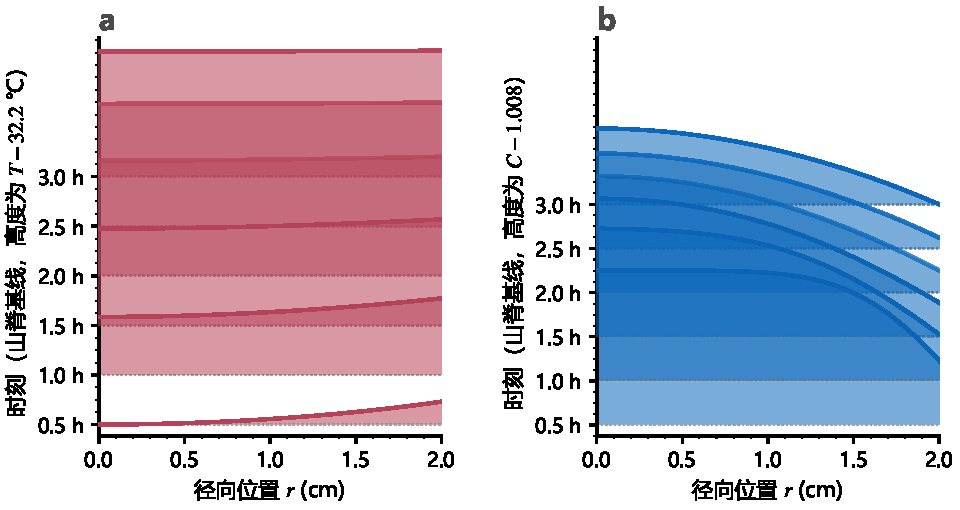
\includegraphics[width=0.9\textwidth,height=0.8\textheight,keepaspectratio]{../figures/fig_q2_ridgeline.pdf}
  \caption{问题 2 径向剖面的山脊图，6 个整时刻沿纵深方向排开（0.5\,h 间隔，
  21 个径向位置），纵向偏移即时间，每条山脊的高度是该时刻剖面相对全场最小值
  的抬升量。a：温度；b：含水率。干燥自表面向内推进，表面与轴线的落差先增大
  后随整体变干而趋缓，最湿位置始终在轴线附近。山脊排布用于避免六条剖面互相压线。}
  \label{fig:q2-ridgeline}
\end{figure}

温度一侧的山脊逐条变平，最后几条几乎成为水平线，对应温度场趋于均匀。含水率一侧的山脊则始终保持自轴线向表面下倾的形状，倾斜程度在第一小时后趋于稳定，说明干燥进入了一个形状大致自相似、整体逐步下移的阶段。所有时刻的最高点都落在轴线一侧，没有出现内部极值或局部反转，这一形态直接决定了下一问判据的取法：既然最湿的位置始终在轴线附近，要判断药材各处是否达标，就必须盯住径向最大值。本问的截面水分总量平衡残差为 $5.5\times10^{-13}$，与问题一同处机器精度量级。
